\section{Algorithmic improvement of PELE}

Most of the limitations of PELE enumerated in the introduction (Section~\ref{sec:anm_limi}) are common to all methods using NMA or more specifically ANM, and therefore not exclusive to PELE. Some of the issues are related to the NMA model itself, while the rest are related to the specific ways normal modes are applied. This made us think that finding an alternative to the NMA algorithm would produce a noticeable improvement in PELE sampling robustness and performance. To this end, we have chosen to implement an internal coordinate (IC) based NMA.

\subsection{Switching to a different coordinates space} 

Internal coordinate NMA (icNMA) is not a novelty. Indeed, the pioneering NMA works of Wilson \cite{wilson_molecular_2012} were already performed in the internal coordinates space. This is not surprising, given that internal coordinates (e.g. bond distance, bond angle, and dihedral torsion angles) are the most natural way of representing chemical molecules (e.g. with a z-matrix \cite{gordon_approximate_1968}). Actually, several methods use internal coordinates instead of Cartesian coordinates. Some examples are the Multiple Minima Monte Carlo \cite{li_monte_1987} method, the Monte Carlo sampling software MCPRO (Monte Carlo for PROteins) \cite{jorgensen_molecular_2005} and ICM \cite{abagyan_icm_1994}, or the MD software X-PLOR \cite{stein_torsion-angle_1997} and DYANA \cite{guntert_torsion_1997}.

The truth is that Cartesian coordinate NMA methods (ccNMA) are more common than icNMA-based methods, possibly because the mathematical background of the former is more simple. However, this fact has not prevented researchers from introducing icNMA in their simulation software. First examples can be found in the early works of Noguti \textit{et al.} \cite{noguti_method_1983, noguti_efficient_1985} and Kidera \textit{et al.} \cite{kidera_enhanced_1995,kidera_smart_1999} where the  scaled collective variables (SCV) MC and related algorithms are presented. Trosset  \textit{et al.} used later a similar methodology \cite{trosset_prodock_1999} in the implementation of PRODOCK. Levitt and Stern \cite{levitt_protein_1985} suggested an MD method using IC NMA modes. Finally, Lin and coworkers \cite{lin_evaluating_2011} developed a different method using icNMA followed by an energy minimization. 

There exist reports claiming that a significantly smaller number of modes are needed to reproduce conformational changes using torsional NMA \cite{bray_optimized_2011}, and that this method improves sampling quality \cite{mendez_torsional_2010-1} and the results of ligand binding simulations \cite{kovacs_conformational_2005} compared to ccNMA-based methods. Changing the coordinate system  implies not only changing the way normal modes are calculated, but also the way modes are applied, which could help to mitigate many of the NMA-related issues.

\subsection{Coarse grain model}
The CG model used in our icNMA implementation describes rigid units that encompass all the heavy atoms among rotatable backbone torsions ($[C_\alpha]^3$ \cite{ghysels_mobile_2009, ghysels_comparative_2010} model). This means that we will define \around$2R$ units for each chain (where $R$ is the number of residues), which can be of 4 different types (see Fig. \ref{fig:icNMA_CG}):

\begin{description}
\item [N-terminal unit] Contains the N-terminus, \calpha and first residue side chain.
\item [\calpha unit] Contains the \calpha atom and side chain.
\item [C-terminal unit] Contains the atoms that form the final carboxyl group.
\item [Peptide bond unit] Contains the carboxyl and amino groups involved in the peptide bond.
\end{description}

To account for the rigidity of the $\phi$ torsion in prolines, its peptide bond and \calpha units will be fused together (see Fig. \ref{fig:icNMA_CG}B).

\begin{figure}
\fittopageimage{CoarseGrainModel}
\caption{CG model of a peptide (A) using the $[C_\alpha]^3$ distribution of atoms. Each residue is composed of two units which are delimited by the $\phi$ and $\psi$ torsions. The case of proline residues (B) is special, as they only form one unit.}
\label{fig:icNMA_CG}
\end{figure}

\subsection{icNMA theory}

\subsubsection{Hessian calculation}

\begin{figure}
\fittopageimage{VectorialNotationANMIC}
\caption{Representation of the rotation of two rigid bodies (green and purple) around axis $q_{\alpha}$.}
\label{fig:icNMA_bodies}
\end{figure}

Again, we model our system as a spring network whose potential is the sum of all Hookean interactions between atoms (or CG units) with the form $Vij = \frac{k_ij}{2} (r_{ij} - r_{ij}^0)$\footnote{As a convention, units and dihedrals will be numbered correlatively from N-terminal to C-terminal. Regular letters will be used to index atoms and units, and Greek letters to index dihedrals.}. If we express these interactions using generalized internal coordinates (which in our case will be limited to the torsion angles of backbone dihedrals), we can write the potential energy as:

\begin{equation}
V = \frac{1}{2} (q - q^0) H (q-q^0)^T
\end{equation}

and the Hessian in terms of $q$ \cite{kovacs_conformational_2005} as:

\begin{equation}
H_{\alpha,\beta} = \frac{\partial^2 V }{\partial q_\alpha \partial q_\beta} = \sum_{i<j} \frac{f_{ij}}{ \left| r_{ij} \right|^2} \left< r_ij , \frac{\partial r_i - \partial r_j}{\partial q_\alpha} \right> . \left< r_ij , \frac{\partial r_i - \partial r_j}{\partial q_\alpha} \right > 
\end{equation}

which depends on the values of the inverse of Wilson's $B$ matrix \cite{wilson_molecular_2012} ( with elements $\frac{\partial r_i}{\partial q_\alpha}$). If we impose Eckart conditions \cite{eckart_studies_1935} ($\sum_i m_i \frac{\partial r_1}{\partial q_\alpha} = 0$  and $\sum_i m_ir_i^0 \times \frac{\partial r_1}{\partial q_\alpha} = 0$ ) and that the origin of the molecule is the center of mass, the partial derivatives can be calculated as \cite{noguti_dynamics_1983}:

\begin{equation}
\frac{\partial r_1}{\partial q_\alpha} = e_\alpha \times \left( \frac{M_2}{M} r_\alpha + \frac{M_1}{M} r_1^0 \right) - r_1 \times \frac{M_1 r_1^0 \times (e_\alpha \times r_\alpha) + I_2 e_\alpha)}{I}
\end{equation}

\begin{equation}
\frac{\partial r_2}{\partial q_\alpha} = - e_\alpha \times \left( \frac{M_1}{M} r_\alpha + \frac{M_2}{M} r_2^0 \right) + r_2 \times \frac{M_2 r_2^0 \times (e_\alpha \times r_\alpha) + I_1 e_\alpha)}{I}
\end{equation}

which describes the change of Cartesian coordinates when one part of the chain is kept fixed and the other part moves around torsion $q_\alpha$ and vice versa. Both rigid bodies must be taken into consideration for a single rotation, as Eckart conditions imply the conservation of momentum. In these and in the following equations, $M$ is the summed mass and $I$ is the inertia tensor for all the units that compose the molecule. $M_1$, $M_2$, $I_1$, $I_2$, $r^0_1$ and $r^0_2$ are the summed masses, inertia tensor and center of mass of the set of units to the left (subindex $1$) or to the right (subindex $2$) of dihedral $q_\alpha$ ; $e_\alpha$ is a unit vector with the direction of the bond;  $r_\alpha$ and $r_{\alpha+1}$ are the positions of the atoms at both ends of the rotatable bond. Finally, $r_1$ and $r_2$ are arbitrary atoms in any of the left or right units of $q_\alpha$ torsion (see Fig. \ref{fig:icNMA_bodies}).

From these equations, a naive expression for the Hessian calculation can be deduced with a $\Theta (n^4)$ computational cost (assuming that the number of dihedrals is roughly proportional to the number of atoms). We are again in debt to Noguti and Go \cite{noguti_method_1983} and Abe and coworkers \cite{abe_rapid_1984} for the development of a recurrent method to calculate the Hessian, which can be implemented as a faster recursive algorithm ($\theta(n^2)$) that also turns out to be more memory efficient. First, Cartesian and internal coordinate-dependent terms are separated so that we can write each Hessian element as

\begin{equation}
H_{\alpha,\beta} = \left( e_\alpha, e_\alpha \times r\alpha \right) R_{\alpha,\beta} \left( \begin{array}{cc} e_\alpha \\\ e_\alpha \times r\alpha \end{array} \right)
\end{equation}

where the matrix $R$ is calculated as 

\begin{equation}
R_{\alpha,\beta} = \sum_i {\scriptscriptstyle \alpha} \sum_j {\scriptscriptstyle \beta} D_{ij}
\end{equation}

$D$ matrix models the interaction of atom $i$ and $j$:

\begin{equation}
D_{ij} = \frac{f_{ij}}{ \left| r_{ij} \right|^2} \left( \begin{array}{cc} r_i \times r_j \\\ r_{ij} \end{array} \right) \left( r_i \times r_j , r_{ij} \right)
\end{equation}

where the distance-dependent force constant is calculated as:

\begin{equation}
f_{ij} = \frac{k_0} { 1.0 + \left( \frac{r_{ij}}{x0} \right) ^6}.
\end{equation}

In our implementation, $k = 1$ and  $x0 = 3.8$, which are the same definitions used by the iNMA software \cite{lopez-blanco_imod_2011}.

To calculate the elements of $R$ we may need to store (or recalculate, which would affect computational efficiency) all $D_{ij}$ values. The number of matrices stored can be lowered by defining a matrix $T$, whose elements $T_{ab}$ summarize the interactions of all the atoms of rigid units $a$ and $b$:

\begin{equation}
T_{a,b} = \sum_{j \in a} \sum_{j \in b} D_{i,j}
\end{equation}

It is possible to calculate $R$ from $T$ by determining a new matrix $U$ so that:

\begin{equation}
U_{ab} = \sum_{i \leq a} \sum_{j >b} T_{ab}
\end{equation}

which contains all atomic interactions from the first unit to the $a$ unit, and from the $b$ unit to the last one (which can be interpreted as fixing units $a$ to $b$ and allowing units 0 to $a$ and $b+1$ to $M$ to rotate along dihedrals $\alpha = a$ and $\beta = b$). This makes it possible to calculate $R$ with only one index change: 

\begin{equation}
R_{\alpha,\beta} = U_{a,b+1}
\end{equation}

Finally, a recursive solution can be written so that:

\begin{equation}
U_{a,b} = U_{a,b+1}+U_{a-1,b} + U_{a-1,b+1}+T_{a,b}
\end{equation}

being the value of $U$ equal to 0 if any of its indexes is outside the range [0, $M$-1].


\subsubsection{Calculation of the metric tensor} 

We can also express the kinetic energy in terms of the generalized coordinates $q$ so that 

\begin{equation}
K = \frac{1}{2} \dot{q}^T K \dot{q}
\end{equation}

and the metric tensor K becomes

\begin{equation}
K_{\alpha,\beta} = \frac{\partial^2 K}{ \partial \dot{q}_\alpha \partial \dot{q}_\beta} = \sum_i^n m_i \left< \frac{\partial r_i}{ \partial q_\alpha} , \frac{\partial r_i}{ \partial q_\beta} \right>
\end{equation}


which can be calculated as \cite{noguti_dynamics_1983}:

\begin{equation}
\begin{split}
K_{\alpha\beta} = \frac{M_1 M_3}{M} \left[ e_\alpha \times (r_\alpha - r^0_1) \right] \left[ e_\beta \times (r_\beta - r^0_3)\right ] + \\ \left[ M_1 r_1^0 \times (e_\alpha \times r_\alpha) - I_1 e_\alpha \right] I^{-1} \left [M_3 r_3^0 \times (e_\beta \times r_\beta) - I_3 e_\beta \right]
\end{split}
\end{equation}


We are currently using the definition of the inertia tensor provided by Noguti and Go \cite{noguti_dynamics_1983}, also employed by Braun \textit{et al.} \cite{braun_formulation_1984} as defined by Lu and coworkers \cite{lu_new_2006} so that

\begin{equation}
I = \sum_i m_i P^T P
\end{equation}

and 

\begin{equation}
P_i = \left( \begin{array}{ccc} 0 & -z & y \\\ z & 0 & -x \\\ -y & x & 0 \end{array} \right)
\end{equation}

Once we have obtained the metric tensor and the Hessian, we can calculate the normal modes using Eq. \ref{eq:eigenproblem}. The resulting eigenvalues are still related to mode frequencies. The meaning of the eigenvectors, however, changes compared to their Cartesian coordinates counterparts; their size decreases from $3N$ to \around$2R$ (where $N$ is the number of atoms or CG units) and each single element $\alpha$ represents a differential rotation around torsion $q_\alpha$. 

In a preliminary study \cite{rincon_munoz_alisis_2014} we were able to demonstrate that the internal coordinate and Cartesian coordinate mode spaces are in good agreement.

\subsection{From internal to Cartesian coordinates and back} 

In order to compare IC modes with CC modes, we convert one coordinate system to the other using the Jacobian ($J$, inverse of Wilson's $B$ matrix) in the equation

\begin{equation}
J_{i,\alpha} = \frac{\partial r_i}{\partial q_\alpha}
\end{equation}

We can calculate Cartesian coordinate displacements from torsional rotations (and thus, from IC modes):

\begin{equation}
\Delta \vec{r}_{i,\alpha} = \sum_{\alpha}^N \vec{J}_{i,\alpha} v_i^\alpha  .
\end{equation}

We can also obtain torsional rotations from Cartesian displacements by using:

\begin{equation}
\Delta \Theta = (J^T M J)^{-1} J^T M \Delta r .
\end{equation}

\subsection{Description of the Internal coordinate NMA-based algorithm}
We have introduced a computationally affordable new IC NMA-based algorithm that aims at providing a fast traversal of the conformational space. The algorithm consists of two independent stages: the backbone perturbation and the side chain perturbation.

The backbone perturbation is implemented as an MC algorithm where each iteration comprises four steps:

\begin{enumerate}

\item  \textbf{Calculation of the target angular increments:} a normal mode and a sense for the rotations is randomly selected. The mode is scaled so that the maximum rotation amplitude is inside a user-defined range. The user can chose to specify a maximum ($a_{max}$) and a  minimum ($a_{min}$) value for the amplitude instead. In this case the maximum amplitude value is sampled from a truncated normal distribution with mean $\nicefrac{ (a_{min} + a_{max})}{2}$ and standard deviation $\nicefrac{(a_{min} - a_{max})}{4}$. Normal modes are calculated only at the beginning of the first iteration.

\item \textbf{Application of the angular increments:} the geometry of the protein is updated using Choi's \cite{choi_updating_2006-1} quaternion method.

\item \textbf{Side chain relaxation:} the rotations in the previous step treat side chains as rigid bodies. This may introduce atom clashes that must be freed. To this end, the side chains with any atom involved in a steric clash are selected and minimized. Note that, as only side chains are minimized, the conformations with clashes involving backbone atoms will be discarded in the next step because of their high potential energy. 

\item \textbf{Acceptance criterion:} the Boltzmann criterion is tested and the new conformation is accepted or rejected. 

\end{enumerate}

The side chain perturbation is again implemented as an MC algorithm where, at each iteration, a side chain is randomly selected and modified. To change the side chain, its rotatable bonds are found and a random increment is applied to each of them. The new side chain conformation will be accepted or rejected depending on the result of the Boltzmann criterion.


\subsection{Alternative implementation}

We also worked on a solution that allowed us to fuse the icNMA step with PELE original scheme \cite{rincon_munoz_alisis_2014} (i.e. performing an icNMA step plus the relaxation phase). As in the regular PELE algorithm, the last minimization must be constrained so that the backbone proposal is maintained. In this case, we have applied harmonic dihedral constraints ($U_{\alpha}^c(q_\alpha) = \nicefrac{k}{2} (q_\alpha-q_\alpha^0)$) to a percentage of the most flexible torsions. Restricting the number of constraints makes it is easier for the minimizer to free backbone stress and it helps it to converge faster. The gradient and Hessian derivations have been calculated and translated to C using the symbolic algebra software Maxima \cite{maxima_maxima_2014}. This alternative was studied during the preliminary development stage providing analogous results to those of ccNMA (the protein was collapsing into a compact form). This lead us to conclude that minimizations had a role in the sampling bias. 

\section{Obtention of the best set of parameters}

To compare IC and CC methods, we first need to obtain the set of parameters that maximizes the performance of both method simulations. To this end, we chose the most relevant parameters for each method and analyzed how their changes were affecting performance.  

\subsection{Characterization of the NMA step}

We started by isolating the mode application procedure in both methods. The ccNMA step comprises two smaller substeps:
\begin{enumerate}
  \item The calculation of the translation vectors, which depends on the \calpha displacement factor parameter (\textit{displacementFactor} defines the maximum displacement for the \calpha atoms).
  \item The application of these translations through a minimization. The ``strength'' or ``intensity'' of this minimization depends mainly on two parameters, the force constant of the spring pulling the \calpha atoms (\textit{steeringForce}) and the root mean square of the gradient (\textit{MinimumRMS}) that modulates the convergence of the minimization. 
\end{enumerate}

In the icNMA case, the NMA step coincides with a whole iteration of the backbone perturbation stage, and is performed in two consecutive substeps:
\begin{enumerate}
  \item The calculation of the torsional increments, which depends on the displacement factor parameter (\textit{displacementFactor}, which, in turn, defines the maximum rotation of any backbone torsional angle).
  \item The application of the rotations, which has no parameter dependencies.
  \item The side chain relaxation step, which again depends on the root mean square of the gradient (\textit{relaxMinimRmsg}).
\end{enumerate}

Table \ref{tab:parameters} summarizes the parameters that govern both methods.

\begin{table}
\centering
\begin{tabular}{ r c c c  }
\toprule
Method  & Movement amplitude & \multicolumn{2}{c}{Minimization strength} \\
\midrule
CC & \specialcell{displacementFactor\\ (\angstrom)} & \specialcell{steeringForce\\ ($kT/\AA$)} &\specialcell{ MinimumRMS \\(\nicefrac{kcal}{mol \angstrom})} \\
~  & 0.25, 0.66, 1.08, 1.5, 1.92 & 20, 40, 60, 80, 100 & 0.01, 0.05, 0.1\\
  IC & \specialcell{displacementFactor\\ (radians)} & \multicolumn{2}{c}{\specialcell{relaxMinimRmsg\\(\nicefrac{kcal}{mol \angstrom})}} \\
~  & 0.02, 0.05, 0.075 ,0.1, 0.12, 0.15 & \multicolumn{2}{c}{0.01, 0.05, 0.1}\\
\bottomrule
\end{tabular}
\caption{Choice of parameters affecting the mode application step in the CC and IC methods, including the values that will be used in characterization tests.} \label{tab:parameters}
\end{table}

To characterize the results of each step, we have focused on three features:
\begin{itemize}
	\item The \calpha RMSD between the initial conformation and the conformation after the mode application step, which shows the extent of the backbone deformation.
	\item The increment of internal energy between the starting conformation and the conformation after the NMA step, which shows how likely this deformation would be.
	\item The time the step takes.
\end{itemize}

Ideally, a good set of parameters is the one that produces big RMSD displacements at a low energy cost.

To study the effect and relevance of our parameter choice, we performed several simulations at 3000 K with a cutoff distance for the EN of 9 \angstrom, random selection of pure modes (which means that modes will not be combined) and different values of movement amplitude and minimization strength (see Table \ref{tab:parameters}. We have used the c-Src kinase structure (PDB id: 1y57) as test system. This protein performs wide inter-domain conformational transitions as well as loop rearrangements involving the temporary creation of secondary structures. As we have seen in Section \ref{sec:supp_mat_cc_vs_c} and Section \ref{sec:anm_limi}, the choice of the initial conformation can give place to very different mode spaces, which has an effect on the conformational search. This is the reason why  we have used two different starting conformations in this test: an open P-loop structure (with a 17.32 \angstrom distance between CYS:277:CA and LEU:387:CA) and a semi-closed P-loop one (with 13.5 \angstrom between the same atoms). Both of them come from previous PELE simulations, which means that they have been previously minimized. The temperature of the simulation ensures high acceptance rates and, therefore, a wider exploration of the conformational space (we have not taken into account the biophysical correctness of the exploration at this point).
 
We run a first set of short CC simulations (\around100 steps) in order to determine which minimization strength parameter we should modify and, therefore, further delimit the number of parameters to analyze. As both \textit{steeringForce} and \textit{MinimumRMS} influence minimization, we decided to fix \textit{steeringForce} to 20 $kT/\AA$ when changing \textit{MinimumRMS}, and \textit{MinimumRMS} to 0.05 \nicefrac{kcal}{mol \angstrom} when changing \textit{steeringForce}. These are commonly used values for these parameters.

The plots in Fig. \ref{fig:cc_300_avg_rmsd_energy} show a strong positive relationship between the \textit{displacementFactor} parameter (colored clusters), the amount of deformation (RMSD) and the energy increment ($\Delta U$). The RMSD averages are similar for both parameters and structures, while the average energy for the simulations where the \textit{steeringForce} is being modified is, in general, higher.  

However, the relationship of the \textit{relaxMinimRmsg} or \textit{steeringForce} with the studied features is not that clear. In order to gain more insight, we measured the association strength of these variables using the Spearman rank correlation. This coefficient can be calculated as 

\begin{equation}
\rho = 1- \frac{6\Sigma d^2_i}{n (n^2-1)},
\end{equation}

where $d$ is the difference between ranks and n is the number of samples. 

The Spearman rank correlation is a non-parametric test that works with ranked ordinal data with monotonic relationships and does not make any assumption about data distribution (e.g. Pearson product-moment correlation assumes distributions to be normal). We consider that coefficients between 0.10 and 0.29 represent a small association; coefficients between 0.30 and 0.49 represent a medium association; and coefficients above 0.50 represent a tight relationship. The results, summarized in Table \ref{tab:rmsg_steering_corr}, confirm that both minimization strength parameters play an important role in the final energy increment. Given this, and the fact that the changes in \textit{steeringForce} produce larger energy averages, we decided to keep this parameter fixed to its default value in the next tests.      

\begin{table}
\centering
\begin{tabular}{ c c c c c }
\toprule
 	\multicolumn{1}{c}{\ }& \multicolumn{2}{c}{Open} & \multicolumn{2}{c}{Closed} \\
\midrule
 	\multicolumn{1}{c}{\ }& steeringForce & MinimumRMS & steeringForce & MinimumRMS \\
	RMSD & \strcolor{0.044} (0.019) & \strcolor{-0.015} (0.421) & \strcolor{0.042} (0.019) & \strcolor{-0.052} (0.004)\\
	$\Delta U$ & \strcolor{0.223} ($<$0.001) & \strcolor{0.180} ($<$0.001) & \strcolor{0.175} ($<$0.001) & \strcolor{0.163} ($<$0.001)\\
\bottomrule
	%Time & \strcolor{0.278} ($<$0.001) & \strcolor{-0.482} ($<$0.001) & \strcolor{0.321} ($<$0.001) & \strcolor{-0.517} ($<$0.001)\\
	%\hline
\end{tabular}
\caption{Association strength of the studied parameters and simulation features. Each value has been colored depending on its category: Green for high association, yellow for medium association, orange for low association and red for no association.} \label{tab:rmsg_steering_corr}
\end{table}

\begin{figure}
	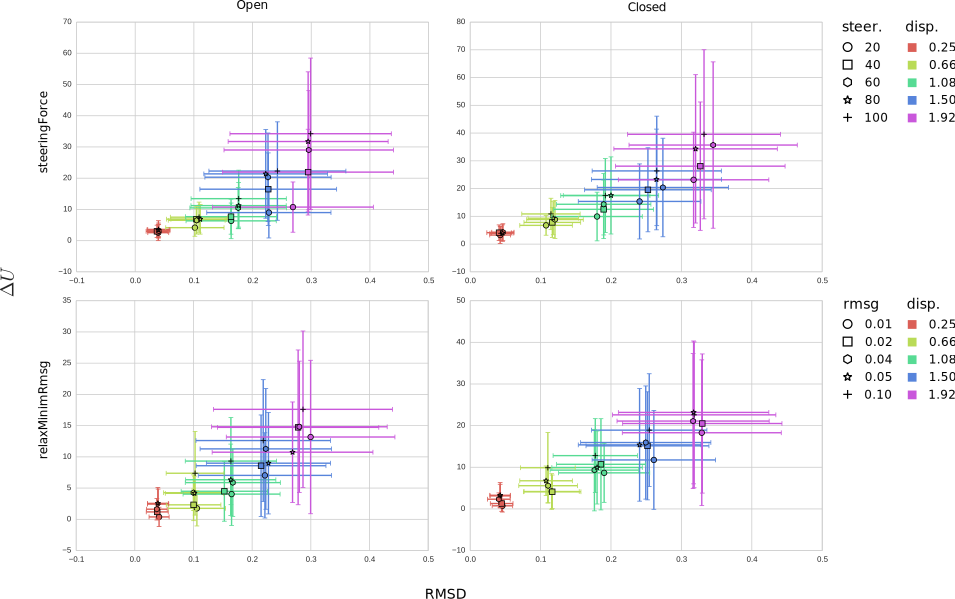
\includegraphics[width=\linewidth, height=\textheight, keepaspectratio]{CC_300_step_avg_rmsd_ener}
	\caption{Plot showing the relationship of the two studied parameters (\textit{steeringForce}  and \textit{MinimumRMS}) with the RMSD and energy increments of the Cartesian coordinate ANM step. Each point shows the average and standard deviation of the RMSD and energy increments for a given combination of parameters.}
	\label{fig:cc_300_avg_rmsd_energy}
\end{figure}

Having discarded to modify the \textit{steeringForce} parameter, we proceeded to perform other longer simulations (\around1500 steps) by varying the remaining parameters. Since the simulations starting from the closed structure looked more static, this time we started all simulations from the open structure. The reason for this behavior could be the higher overlap of the open conformation modes with the open to close transition. The simulations have been performed using temperatures between 300 K and 2568 K and the Spearman rank correlation for the (computational) step time, energy and RMSD increments (always of the NMA step) has been calculated (see Table \ref{tab:nma_correlations}).      

\begin{center}
\begin{longtable}{r r c c c c}


\toprule
~ & ~ & \multicolumn{2}{c}{CC} & \multicolumn{2}{c}{IC}\\
T & ~ & $\rho$ & p-value & $\rho$ & p-value \\
\midrule

300 & RMSD {\textbackslash} $\Delta U$ &  
\strcolor{0.79} &
$<$0.001 &
 \strcolor{0.69} &
$<$0.001\\
 &
Step time {\textbackslash} Displacement &
 \strcolor{0.563} &
$<$0.001 &
 \strcolor{0.615} &
$<$0.001\\
 &
Step time {\textbackslash} Relax. strength &
 \strcolor{-0.591} &
$<$0.001 &
 \strcolor{0.002} &
 0.783\\
 &
RMSD {\textbackslash} Displacement &
 \strcolor{0.786} &
$<$0.001 &
 \strcolor{0.78} &
$<$0.001\\
 &
RMSD {\textbackslash} Relax. strength &
 \strcolor{-0.057} &
$<$0.001 &
 \strcolor{-0.003} &
 0.594\\
 &
$\Delta U$ {\textbackslash} Displacement &
 \strcolor{0.656} &
$<$0.001 &
 \strcolor{0.717} &
$<$0.001\\
 &
$\Delta U$ {\textbackslash} Relax. strength &
 \strcolor{0.214} &
$<$0.001 &
 \strcolor{-0.005} &
 0.405\\
 \hline
 583 &
RMSD {\textbackslash} $\Delta U$ &
 \strcolor{0.79} &
$<$0.001 &
 \strcolor{0.63} &
$<$0.001\\
 &
Step time {\textbackslash} Displacement &
 \strcolor{0.548} &
$<$0.001 &
 \strcolor{0.591} &
$<$0.001\\
 &
Step time {\textbackslash} Relax. strength &
\strcolor{-0.598} &
$<$0.001 &
 \strcolor{-0.006} &
 0.274\\
 &
RMSD {\textbackslash} Displacement &
 \strcolor{0.803} &
$<$0.001 &
 \strcolor{0.785} &
$<$0.001\\
 &
RMSD {\textbackslash} Relax. strength &
 \strcolor{-0.051} &
$<$0.001 &
 \strcolor{0.001} &
 0.895\\
 &
$\Delta U$ {\textbackslash} Displacement &
\strcolor{ 0.66} &
$<$0.001 &
 \strcolor{0.659} &
$<$0.001\\
 &
$\Delta U$ {\textbackslash} Relax. strength &
 \strcolor{0.213} &
$<$0.001 &
 \strcolor{0.007} &
 0.216\\
\midrule
 866 &
RMSD {\textbackslash} $\Delta U$ &
 \strcolor{0.79} &
$<$0.001 &
 \strcolor{0.6} &
$<$0.001\\
 &
Step time {\textbackslash} Displacement &
 \strcolor{0.562} &
$<$0.001 &
 \strcolor{0.588} &
$<$0.001\\
 &
Step time {\textbackslash} Relax. strength &
 \strcolor{-0.605} &
$<$0.001 &
 \strcolor{0.001} &
 0.808\\
 &
RMSD {\textbackslash} Displacement &
 \strcolor{0.794} &
$<$0.001 &
 \strcolor{0.788} &
$<$0.001\\
 &
RMSD {\textbackslash} Relax. strength &
 \strcolor{-0.03} &
$<$0.001 &
 \strcolor{-0.005} &
 0.374\\
 &
$\Delta U$ {\textbackslash} Displacement &
 \strcolor{0.656} &
$<$0.001 &
 \strcolor{0.629} &
$<$0.001\\
 &
$\Delta U$ {\textbackslash} Relax. strength &
 \strcolor{0.195} &
$<$0.001 &
 \strcolor{0.011} &
 0.059\\
\midrule
 1150 &
RMSD {\textbackslash} $\Delta U$ &
 \strcolor{0.79} &
$<$0.001 &
 \strcolor{0.58} &
$<$0.001\\
 &
Step time {\textbackslash} Displacement &
 \strcolor{0.569} &
$<$0.001 &
 \strcolor{0.618} &
$<$0.001\\
 &
Step time {\textbackslash} Relax. strength &
 \strcolor{-0.579} &
$<$0.001 &
 \strcolor{0.002} &
 0.753\\
 &
RMSD {\textbackslash} Displacement &
 \strcolor{0.799} &
$<$0.001 &
 \strcolor{0.79} &
$<$0.001\\
 &
RMSD {\textbackslash} Relax. strength &
 \strcolor{-0.033} &
$<$0.001 &
 \strcolor{0.005} &
 0.372\\
 &
$\Delta U$ {\textbackslash} Displacement &
 \strcolor{0.65} &
$<$0.001 &
 \strcolor{0.607} &
$<$0.001\\
 &
$\Delta U$ {\textbackslash} Relax. strength &
 \strcolor{0.182} &
$<$0.001 &
 \strcolor{0.003} &
 0.603\\
\midrule
 1432 &
RMSD {\textbackslash} $\Delta U$ &
 \strcolor{0.79} &
$<$0.001 &
 \strcolor{0.56} &
$<$0.001\\
 &
Step time {\textbackslash} Displacement &
 \strcolor{0.543} &
$<$0.001 &
 \strcolor{0.579} &
$<$0.001\\
 &
Step time {\textbackslash} Relax. strength &
 \strcolor{-0.609} &
$<$0.001 &
 \strcolor{-0.016} &
 0.006\\
 &
RMSD {\textbackslash} Displacement &
 \strcolor{0.787} &
$<$0.001 &
 \strcolor{0.79} &
$<$0.001\\
 &
RMSD {\textbackslash} Relax. strength &
 \strcolor{-0.046} &
$<$0.001 &
 \strcolor{-0.005} &
 0.38\\
 &
$\Delta U$ {\textbackslash} Displacement &
 \strcolor{0.656} &
$<$0.001 &
 \strcolor{0.589} &
$<$0.001\\
 &
$\Delta U$ {\textbackslash} Relax. strength &
 \strcolor{0.187} &
$<$0.001 &
 \strcolor{0.001} &
 0.822\\
\midrule
 2000 &
RMSD {\textbackslash} $\Delta U$ &
 \strcolor{0.75} &
$<$0.001 &
 \strcolor{0.53} &
$<$0.001\\
 &
Step time {\textbackslash} Displacement &
 \strcolor{0.563} &
$<$0.001 &
 \strcolor{0.559} &
$<$0.001\\
 &
Step time {\textbackslash} Relax. strength &
 \strcolor{-0.566} &
$<$0.001 &
 \strcolor{0.003} &
 0.608\\
 &
RMSD {\textbackslash} Displacement &
 \strcolor{0.782} &
$<$0.001 &
 \strcolor{0.791} &
$<$0.001\\
 &
RMSD {\textbackslash} Relax. strength &
 \strcolor{-0.044} &
$<$0.001 &
 \strcolor{0.001} &
 0.884\\
 &
$\Delta U$ {\textbackslash} Displacement &
 \strcolor{0.615} &
$<$0.001 &
 \strcolor{0.561} &
$<$0.001\\
 &
$\Delta U$ {\textbackslash} Relax. strength &
 \strcolor{0.198} &
$<$0.001 &
 \strcolor{0.008} &
 0.169\\
\midrule
 2568 &
RMSD {\textbackslash} $\Delta U$ &
 \strcolor{0.75} &
$<$0.001 &
 \strcolor{0.51} &
$<$0.001\\
 &
Step time {\textbackslash} Displacement &
 \strcolor{0.57} &
$<$0.001 &
 \strcolor{0.395} &
$<$0.001\\
 &
Step time {\textbackslash} Relax. strength &
 \strcolor{-0.556} &
$<$0.001 &
 \strcolor{-0.046} &
$<$0.001\\
 &
RMSD {\textbackslash} Displacement &
 \strcolor{0.784} &
$<$0.001 &
 \strcolor{0.792} &
$<$0.001\\
 &
RMSD {\textbackslash} Relax. strength &
 \strcolor{-0.047} &
$<$0.001 &
 \strcolor{0.002} &
 0.707\\
 &
$\Delta U$ {\textbackslash} Displacement &
 \strcolor{0.598} &
$<$0.001 &
 \strcolor{0.53} &
$<$0.001\\
 &
$\Delta U$ {\textbackslash} Relax. strength &
 \strcolor{0.199} &
$<$0.001 &
 \strcolor{-0.003} &
 0.547\\
\bottomrule

\caption{Association strenght of the RSMD and energy increments, and step time between themselves and the chosen parameters. }\\
\label{tab:nma_correlations}\\

\end{longtable}

\end{center}

The results show a strong association between the RMSD increment and the energy increment. This is somewhat expected, as big deformations can, in the CC case, distort the topology and, in the IC case, produce more steric clashes. It is remarkable, however, that the association strength is always smaller for the icNMA step, supporting our hypothesis that the icNMA method is able to deform the protein producing smaller energy increments. In this last case we see a slight anticorrelation with the temperature. This is surprising, since all these measures have been taken inside the NMA step and, thus, may be independent of the temperature. 
%\hl{Possible hypotheses for this are: faster sampling of non harmonic regions, or the appearance of multiple pathways, etc., which are associated to a smoother energy landscape in the IC representation.}  

RMSD increments have a strong association with the displacement magnitude, as expected, and no association with relaxation strength in both cases. The energy increment during the NMA step and the displacement magnitude are strongly associated, the explanation behind this is the same that relates RMSD and energy increment. Energy increment and relaxation strength have a loose association in the ccNMA method. This relationship does not exist in the IC case, showing that early convergence should be enough to get rid of steric clashes. All these measures seem to be independent of the temperature.
 
The computational time needed to fulfil the NMA step is, in both cases, strongly related to the displacement magnitude. The reasons are different for each method: In the ccNMA step, the more distant the target positions are, the more difficult the convergence of the minimization becomes, as it has to fulfill the force field constraints plus the ANM constraints. In the icNMA case, the wider the rotation is, the easier it is to generate steric clashes, which are harder to relieve using the minimization. 

Finally, we can observe that the computational time the ccNMA needs to perform a step is also strongly associated with the ANM minimization strength, while this association is almost nonexistent in the IC case, giving us more freedom to change the value of this parameter without time penalties.  

\subsection{Obtention of the best simulations and comparison with MD}
One of the goals of this project is to evaluate to which extent the icNMA implementation improves PELE sampling capabilities. To this end, we have decided to compare simulations using both methods with a third reference method: MD. We have tested two different systems, ubiquitin (PDB id: 1UBQ) a small and very static globular protein,  and a c-Src kinase (PDB id: 1Y57) as an example of a bigger and more flexible protein.

\subsubsection{Best values for the parameters at 300 K} 
The value of the parameters used in a simulation can dramatically alter its outcome. As the icNMA-based method is new, and the ccNMA-based method is not  commonly used at 300, we do not have a predefined set of default values for the parameters to use in the simulations. As a consequence, we have worked to obtain the best parameterizations in order to make the comparison fairer. Here, we will illustrate the procedure we followed for the parameterization of the c-Src kinase simulation.
 
First, we have fixed the parameters common to both methods e.g. the temperature was set to 300 K and the distance cutoff for the construction of the EN was set to 9 \angstrom. Then, using the simulations we had already run with the parameters detailed in Table \ref{tab:parameters}, we have calculated the values of the three indices we were going to use to discriminate the best values for the parameters: 

\begin{itemize}
\item The average RMSD increment of the ANM step, which gives us an idea of the extent of the deformations.
\item The root mean square of the root mean square fluctuations (RMSF) for each simulation vs. the RMSF of the MD simulation. This can tell us if the flexibility of our simulations resemble that of the MD simulations.
\item The acceptance, which we wanted to keep in the 20-40\% range.  
\end{itemize}

After applying the acceptance restriction, the list of possible parameterizations went down to three possibilities for each of the simulations (see Table \ref{tab:nma_sim_parameters}) and we were able to choose a good set of parameters for the regular PELE simulations: 0.66 \angstrom for the \textit{displacementFactor} parameter and 0.1 for the \textit{MinimumRMS} parameter. Note that, as results are so similar, we decided to select the higher value of \textit{MinimumRMS}, as we knew it would shorten the execution time of each step. 

For the icNMA method, we saw a high difference in acceptance between the simulations with \textit{displacementFactor} equal to 0.05 rad and \textit{displacementFactor} equal to 0.08 rad, indicating that our angular step choice was too big. To verify this, we refined the icNMA simulations using values of the \textit{displacementFactor} between 0.05 rad and 0.08 rad. The optimum value turned to be around the 0.065 rad. As the method uses a maximum and minimum value for the rotations, we performed further tests using values around 0.065 rad. as the lower limit and an arbitrary maximum value of 0.02 rad. The best combination we found was the range from 0.07 rad to 0.14 rad. 

\begin{table}
\centering
\begin{tabular}{r c c c c c}
\toprule
~ & Acceptance & RMS(RMSF) & RMSD & Disp. mag. (\angstrom) & Rel. str.\\
\midrule
CC & 0.316 & 2.467 & 0.094 & 0.66 &0.05\\
~ & 0.308 & 2.492 & 0.098 & 0.66 &0.01\\
~ & 0.281 & 2.447 & 0.09 & 0.66 &0.1\\
\midrule
IC & 0.334 & 2.618 & 0.126 & 0.5 &0.05\\
~ & 0.328 & 2.642 & 0.127 & 0.5 &0.1\\
~ & 0.298 & 2.651 & 0.126 & 0.5 &0.01\\
\midrule
IC & 0.296 & 2.637 & 0.139 & 0.55 &0.1\\
(refinement) & 0.295 & 2.639 & 0.137 & 0.55 &0.05\\
~ & 0.29 & 2.635 & 0.138 & 0.55 &0.01\\
~ & 0.284 & 2.629 & 0.148 & 0.6  &0.1\\
~ & 0.264 & 2.63 & 0.149 & 0.6  &0.01\\
~ & 0.26 & 2.588 & 0.165 & 0.65 &0.05\\
~ & 0.249 & 2.608 & 0.168 & 0.65 &0.01\\
~ & 0.248 & 2.614 & 0.153 & 0.6  &0.05\\
~ & 0.245 & 2.612 & 0.164 & 0.65 &0.1\\
~ & 0.229 & 2.592 & 0.179 & 0.7  &0.01\\
\bottomrule
\end{tabular}


\caption{Values for the parameters that produced simulations with acceptance between 20 and 40\%.}
\label{tab:nma_sim_parameters}
\end{table}

Once we got the best parameter choice for the icNMA step, we still needed to parameterize the rotation amplitude range of the side chain perturbation step. To this end, we performed several simulations using different values for the maximum and minimum rotation and choosing those which yield acceptance values between 20 and 40\%. The optimum range happened to be 0.02 to 0.024 radians.

\section{Comparison with MD}
We performed 12 independent 24 h simulations for each method and compared different measurements with MD. These measurements include:

\begin{description}

\item [Energy increments]
The increments of the potential energy due to the NMA step perturbation.  

\item [SASA and radius of gyration]
The SASA measures the area of the protein accessible to the solvent, while the radius of gyration calculates the dispersion of the atoms to its center of mass. Both measurements are related to the compactness of the protein.

\item [RMSF]
The RMSF is a measure of the fluctuation per residue (\calpha atom). We expect that similar methods produce similar conformational ensembles and, therefore, similar RMSF profiles. However, it is not guaranteed that two different conformational ensembles have different RMSF profiles. That is why we must combine this measure with others in order to have a real picture of the ensembles/methods similarity.      

\item [Conformational space overlap]
We used a similar approach to the ones shown by Lyman \textit{et al.} \cite{lyman_ensemble-based_2006} and Lindorff-Larsen \cite{lindorff-larsen_similarity_2009} to calculate the extension of the exploration in the conformational space overlap. This strategy consists in clustering the structures of all the methods together using a geometrical distance measure (RMSD). Then the square root of the Jensen-Shannon divergence of the cluster populations (converted to a probability distribution) is calculated, yielding the desired overlap value.
\end{description}

\subsection{Advantages of the new method}
We have observed that the ccNMA step is not able to generate energetically favorable proposals, i.e. proposals that maintain or lower the potential energy and thus will be accepted by means of a Boltzmann criterion. This is, indeed, the reason that makes the relaxation phase a necessary part of the PELE approach. The icNMA algorithm, however, is able to generate energetically favorable proposals \around18-27\% of the times and therefore does not need the computationally costly relaxation step. As a consequence, the icNMA-based algorithm is able to generate MC proposals faster than the ccNMA approach (\around5-7x), while keeping similar RMSD increments.   

The measurements of the SASA and radius of gyration for both algorithms reveal a tendency towards generating more compact structures than MD. This is not unexpected, as our methods use implicit solvent, which is known to produce a bias in favor of compact structures \cite{onufriev_exploring_2004, chen_implicit_2008, zhang_residual_2012}, while our reference MD simulations were run in explicit solvent. There is a remarkable difference between the results for icNMA and ccNMA, being the former in better accordance with MD. The increased compaction of the ccNMA-based algorithm seems to be caused by the repeatedly use of minimizations, which enforce the solvent bias. The absence of backbone minimizations in the icNMA method limits the severity of the bias.  

We also studied the relative fluctuations of the residues by scaling the RMSF profiles and superimposing them. The RMSF profiles of the icNMA method show, in general, good agreement with MD. The ccNMA method shows a poorer performance in the ubiquitin case, specially in the $\beta2$-$\alpha$-helix and the $\beta$4-$\beta$5 loop regions. 

The study of the conformational space overlap shows that, in general, the icNMA-based method is populating regions of the conformational space closer to MD than to the ccNMA-method. Besides, we performed additional analyses of the sampling of the c-Src kinase P-loop. Correctly sampling this loop is of crucial importance as it is involved in the binding mechanisms of the kinase \cite{boggon_structure_2004}. We measured the distances between the atoms CYS:277:CA and LEU:387:CA, which is related to the inter-domain distance and the P-loop sampling. The icNMA algorithm is able to sample a similar range of distances to MD, however, ccNMA rapid compaction prevents it from obtaining similarly good results. This highlights the advantage of the icNMA method, which is less prone to get trapped in energy minima corresponding to compact structures.

\section[Limitations and perspectives]{Limitations of the new method and future perspectives}

In general, we observed that the RMSF baselines of the NMA-based methodologies is always lower  MD baselines. This points to the main limitations of the new method: the lack of anharmonic backbone movements and mapping higher (local) frequency modes, which reduces the amplitude of fluctuations. We wonder if this could be overcome by using IC Principal Component Analysis (PCA) modes, which are known to have a higher anharmonic component \cite{hayward_harmonic_1994}. Also, both methods show high RMSD differences with the structures coming from the MD trajectories. This differences are more evident in the ubiquitin case, where the flexibility of the protein is concentrated on the loops connecting the secondary structure. The cause of these RMSD differences reflects, indeed, the inability of our set of low-frequency NMA modes to model the high-frequency movements occurring in these loops. 

We are currently working to yet lower the execution times and keep improving the simulation flexibility. Our aim is to make this method a good alternative to current VHTS software by finding a good trade off between simulation detail and speed. Moreover, by coupling this procedure with a ligand perturbation step, as done in the PELE algorithm, local fluctuations (not present in the NMA) can be recovered through the response of the protein to the ligand move. We believe that the improvements in simulation reliability shown here can suppose a gain in the long term. Although it is true that it involves a considerable increase in the calculation times, it can save time (and money) at a later stage of the drug discovery process by the early elimination of false positives and negatives.

\newpage
